% Options for packages loaded elsewhere
% Options for packages loaded elsewhere
\PassOptionsToPackage{unicode}{hyperref}
\PassOptionsToPackage{hyphens}{url}
\PassOptionsToPackage{dvipsnames,svgnames,x11names}{xcolor}
%
\documentclass[
  letterpaper,
  DIV=11,
  numbers=noendperiod]{scrartcl}
\usepackage{xcolor}
\usepackage{amsmath,amssymb}
\setcounter{secnumdepth}{-\maxdimen} % remove section numbering
\usepackage{iftex}
\ifPDFTeX
  \usepackage[T1]{fontenc}
  \usepackage[utf8]{inputenc}
  \usepackage{textcomp} % provide euro and other symbols
\else % if luatex or xetex
  \usepackage{unicode-math} % this also loads fontspec
  \defaultfontfeatures{Scale=MatchLowercase}
  \defaultfontfeatures[\rmfamily]{Ligatures=TeX,Scale=1}
\fi
\usepackage{lmodern}
\ifPDFTeX\else
  % xetex/luatex font selection
\fi
% Use upquote if available, for straight quotes in verbatim environments
\IfFileExists{upquote.sty}{\usepackage{upquote}}{}
\IfFileExists{microtype.sty}{% use microtype if available
  \usepackage[]{microtype}
  \UseMicrotypeSet[protrusion]{basicmath} % disable protrusion for tt fonts
}{}
\makeatletter
\@ifundefined{KOMAClassName}{% if non-KOMA class
  \IfFileExists{parskip.sty}{%
    \usepackage{parskip}
  }{% else
    \setlength{\parindent}{0pt}
    \setlength{\parskip}{6pt plus 2pt minus 1pt}}
}{% if KOMA class
  \KOMAoptions{parskip=half}}
\makeatother
% Make \paragraph and \subparagraph free-standing
\makeatletter
\ifx\paragraph\undefined\else
  \let\oldparagraph\paragraph
  \renewcommand{\paragraph}{
    \@ifstar
      \xxxParagraphStar
      \xxxParagraphNoStar
  }
  \newcommand{\xxxParagraphStar}[1]{\oldparagraph*{#1}\mbox{}}
  \newcommand{\xxxParagraphNoStar}[1]{\oldparagraph{#1}\mbox{}}
\fi
\ifx\subparagraph\undefined\else
  \let\oldsubparagraph\subparagraph
  \renewcommand{\subparagraph}{
    \@ifstar
      \xxxSubParagraphStar
      \xxxSubParagraphNoStar
  }
  \newcommand{\xxxSubParagraphStar}[1]{\oldsubparagraph*{#1}\mbox{}}
  \newcommand{\xxxSubParagraphNoStar}[1]{\oldsubparagraph{#1}\mbox{}}
\fi
\makeatother


\usepackage{longtable,booktabs,array}
\newcounter{none} % for unnumbered tables
\usepackage{calc} % for calculating minipage widths
% Correct order of tables after \paragraph or \subparagraph
\usepackage{etoolbox}
\makeatletter
\patchcmd\longtable{\par}{\if@noskipsec\mbox{}\fi\par}{}{}
\makeatother
% Allow footnotes in longtable head/foot
\IfFileExists{footnotehyper.sty}{\usepackage{footnotehyper}}{\usepackage{footnote}}
\makesavenoteenv{longtable}
\usepackage{graphicx}
\makeatletter
\newsavebox\pandoc@box
\newcommand*\pandocbounded[1]{% scales image to fit in text height/width
  \sbox\pandoc@box{#1}%
  \Gscale@div\@tempa{\textheight}{\dimexpr\ht\pandoc@box+\dp\pandoc@box\relax}%
  \Gscale@div\@tempb{\linewidth}{\wd\pandoc@box}%
  \ifdim\@tempb\p@<\@tempa\p@\let\@tempa\@tempb\fi% select the smaller of both
  \ifdim\@tempa\p@<\p@\scalebox{\@tempa}{\usebox\pandoc@box}%
  \else\usebox{\pandoc@box}%
  \fi%
}
% Set default figure placement to htbp
\def\fps@figure{htbp}
\makeatother





\setlength{\emergencystretch}{3em} % prevent overfull lines

\providecommand{\tightlist}{%
  \setlength{\itemsep}{0pt}\setlength{\parskip}{0pt}}



 


\usepackage{xcolor}
\pagecolor[HTML]{1E1E1E}
\color[HTML]{F5F5F5}
\KOMAoption{captions}{tableheading}
\makeatletter
\@ifpackageloaded{caption}{}{\usepackage{caption}}
\AtBeginDocument{%
\ifdefined\contentsname
  \renewcommand*\contentsname{Table of contents}
\else
  \newcommand\contentsname{Table of contents}
\fi
\ifdefined\listfigurename
  \renewcommand*\listfigurename{List of Figures}
\else
  \newcommand\listfigurename{List of Figures}
\fi
\ifdefined\listtablename
  \renewcommand*\listtablename{List of Tables}
\else
  \newcommand\listtablename{List of Tables}
\fi
\ifdefined\figurename
  \renewcommand*\figurename{Figure}
\else
  \newcommand\figurename{Figure}
\fi
\ifdefined\tablename
  \renewcommand*\tablename{Table}
\else
  \newcommand\tablename{Table}
\fi
}
\@ifpackageloaded{float}{}{\usepackage{float}}
\floatstyle{ruled}
\@ifundefined{c@chapter}{\newfloat{codelisting}{h}{lop}}{\newfloat{codelisting}{h}{lop}[chapter]}
\floatname{codelisting}{Listing}
\newcommand*\listoflistings{\listof{codelisting}{List of Listings}}
\makeatother
\makeatletter
\makeatother
\makeatletter
\@ifpackageloaded{caption}{}{\usepackage{caption}}
\@ifpackageloaded{subcaption}{}{\usepackage{subcaption}}
\makeatother
\usepackage{bookmark}
\IfFileExists{xurl.sty}{\usepackage{xurl}}{} % add URL line breaks if available
\urlstyle{same}
\hypersetup{
  pdftitle={Electrochemistry Basics},
  colorlinks=true,
  linkcolor={blue},
  filecolor={Maroon},
  citecolor={Blue},
  urlcolor={Blue},
  pdfcreator={LaTeX via pandoc}}


\title{Electrochemistry Basics}
\author{}
\date{2021-10-16}
\begin{document}
\maketitle


\subsection{Balancing Redox
Half-Reactions}\label{balancing-redox-half-reactions}

\begin{itemize}
\tightlist
\item
  Balancing the main element
\item
  Balancing oxygen by adding water molecules \(H_2O\)
\item
  Balancing hydrogen with Hydronium \(H^+\)
\end{itemize}

The \textbf{anode} \(\rightarrow\) where \textbf{oxidation} happens The
\textbf{cathode} \(\rightarrow\) where \textbf{reduction} happens

There is no link between electrode polarity and whether it's an anode or
cathode. Generator (battery or accumulator) \(\rightarrow\) + is the
cathode, Electrolysis \(\rightarrow\) + is the anode

\subsection{Reference Electrodes}\label{reference-electrodes}

Because only potential \emph{differences} are measured, reference
electrodes are used.

The ideal \emph{Standard Hydrogen Electrode (SHE)} has a 0V potential at
all temperatures, it's defined by the couple \(H^+ / H_2\) (STD: 1 bar
pressure perfect gas and a \(H^+\) concentration of
\(1\ \text{mol.L}^{-1}\)). This redox reaction occurs at a platinized
\href{https://en.wikipedia.org/wiki/Platinum}{platinum} electrode. The
electrode is dipped in an acidic solution and pure hydrogen gas is
bubbled through it. The concentration of both the reduced form and
oxidized form is maintained at unity.

\[
2 H^+_{(aq)} + 2 e^− → H_{2(g)}
\]

The \emph{Normal Hydrogen Electrode}\footnote{Debatable --- ``normal''
  is the old name for ``standard'' in France.} is the closest real
electrode to the SHE with identical pressure and concentration. Its
potential is \(6\text{mV}/\)SHE, the concentration needs to be slightly
higher to approximate SHE even further.

\emph{Calomel Electrode:}

The calomel electrode is a type of half-cell in which the electrode is
mercury coated with calomel (\(\text{Hg}_2\text{Cl}_2\)) and the
electrolyte is a solution of potassium chloride and saturated calomel.

The electrode reaction is:

\pandocbounded{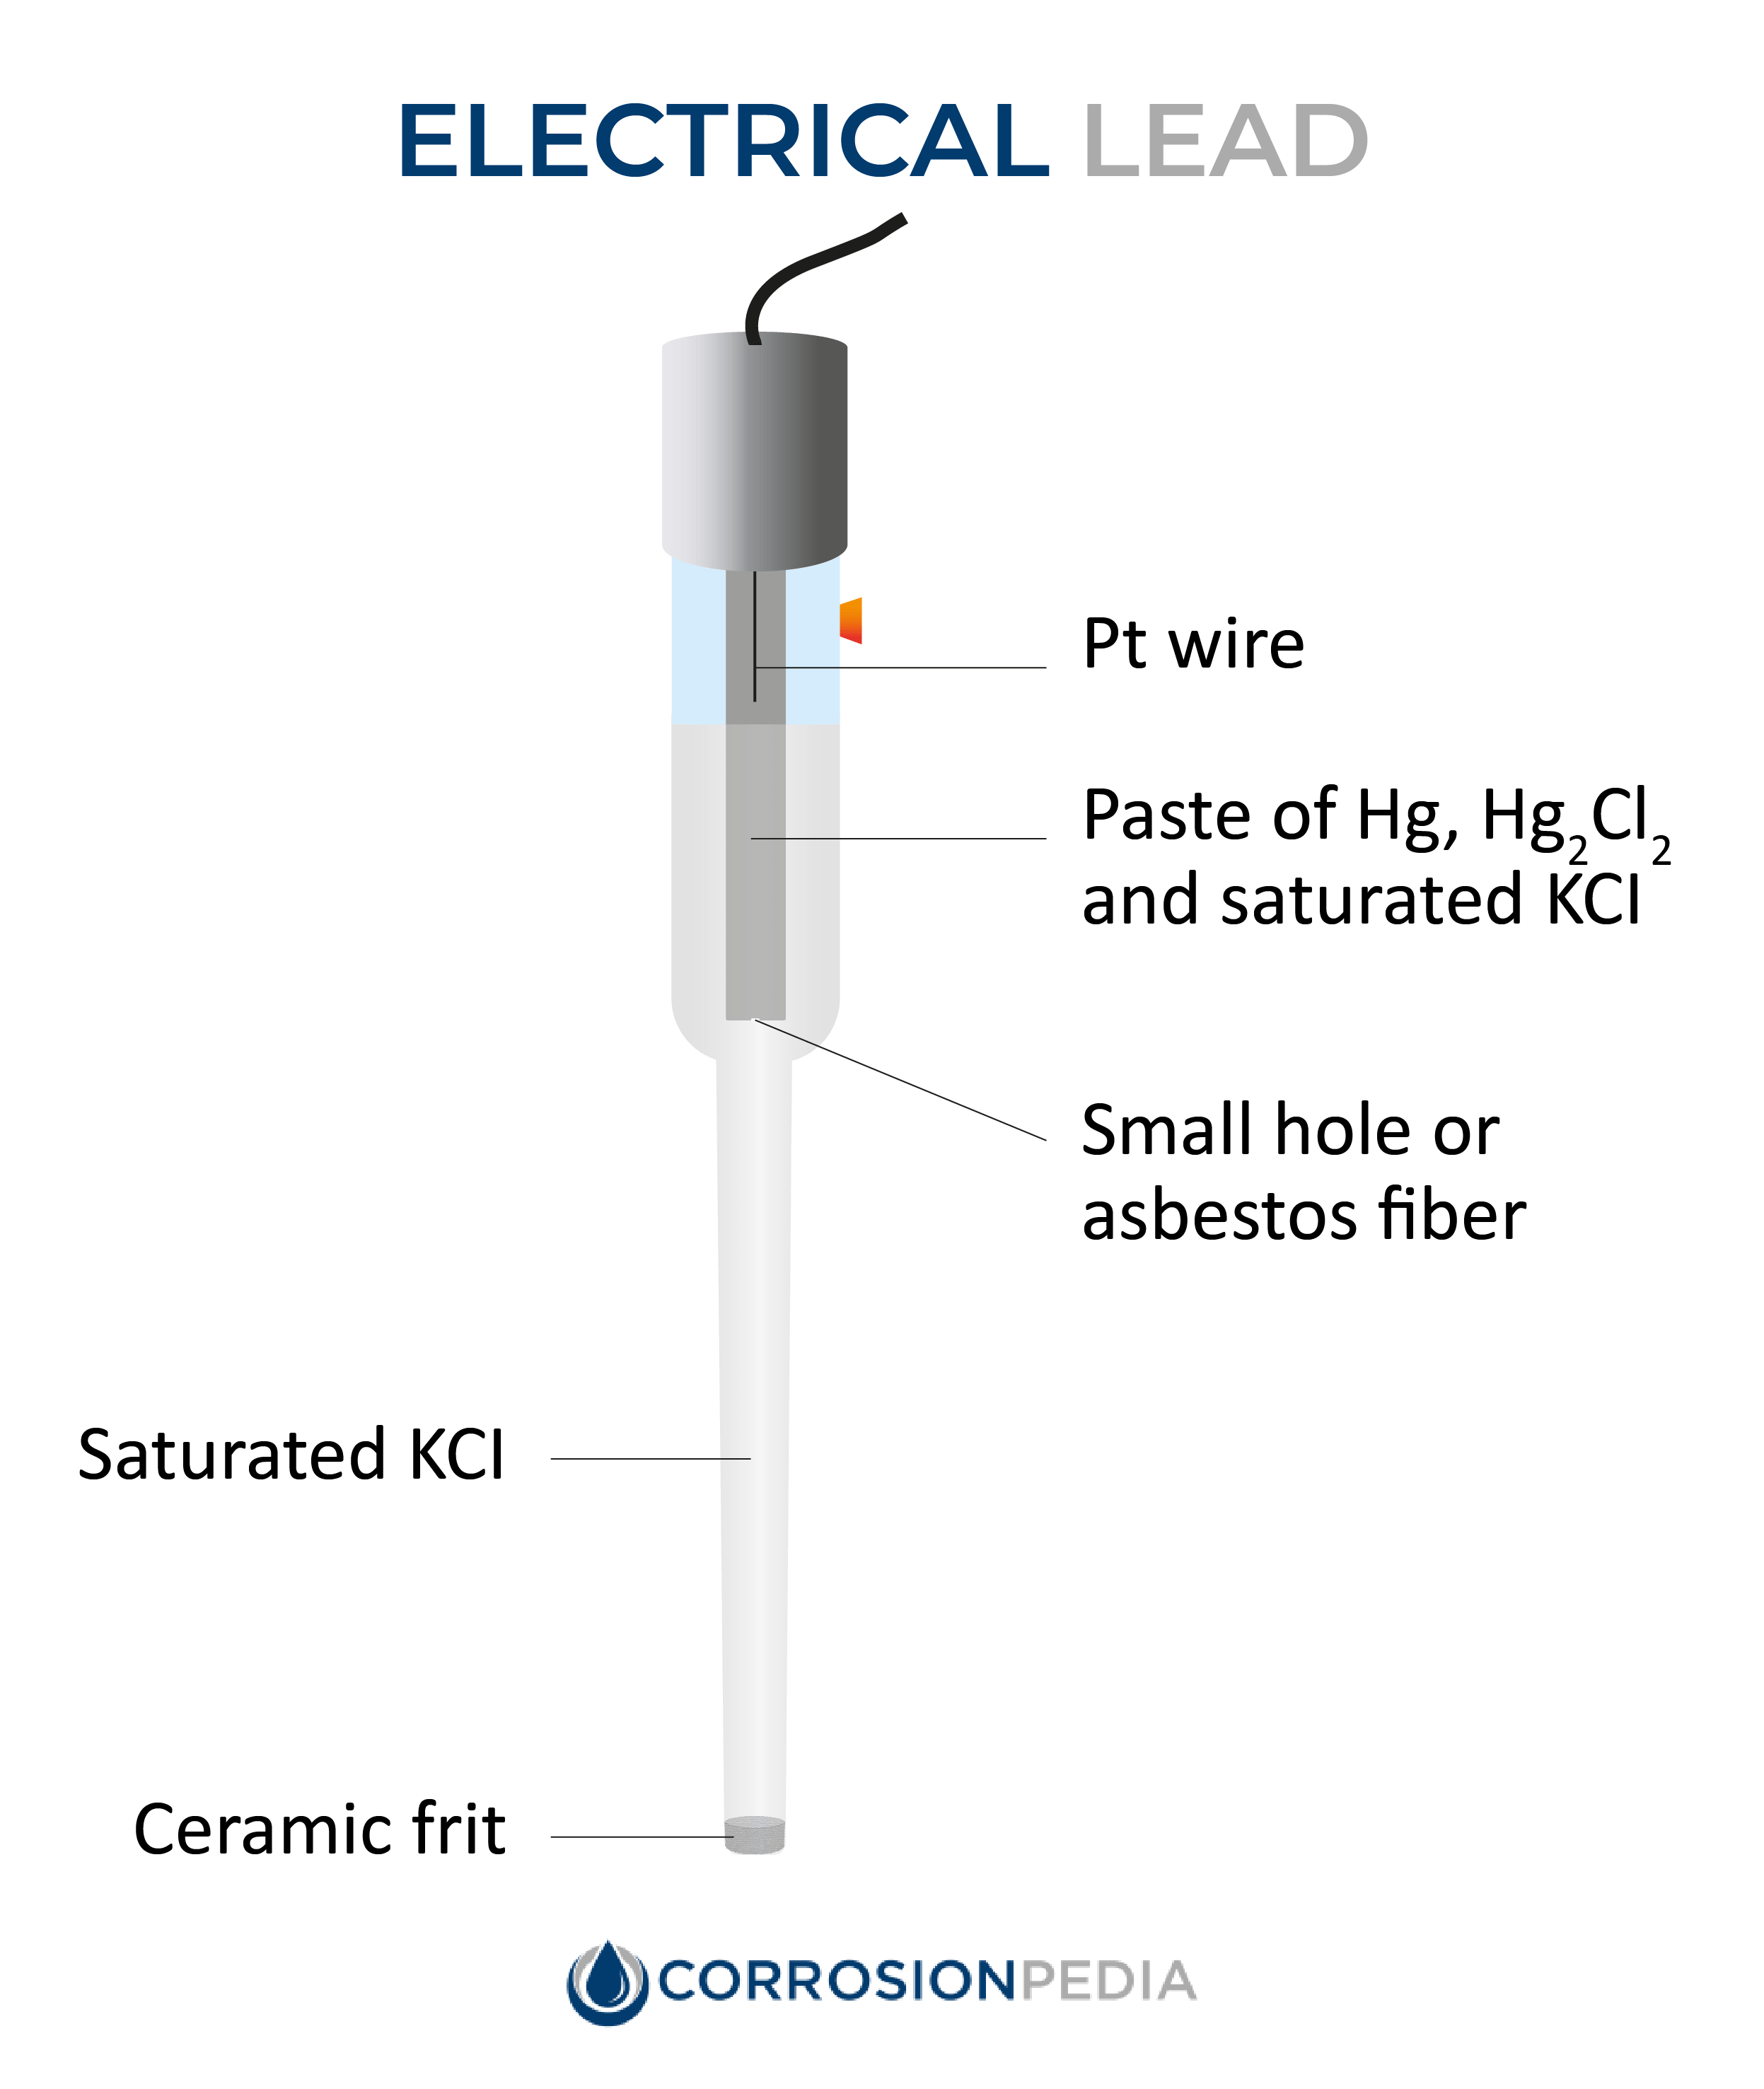
\includegraphics[keepaspectratio]{index_files/mediabag/bc90e3a5-fdc1-4ce6-a.png}}

\[
\text{Hg}^{2+}_2 + 2e^- \leftrightharpoons 2\text{Hg(l)}, \qquad E^0_{\text{Hg}^{2+}_2 / \text{Hg}} = +0.80\text{V}
\]

\[
\text{Hg}_2\text{Cl}_2 + 2e^- \leftrightharpoons 2\text{Hg(l)} + 2 \text{Cl}^-, \qquad E^0_{\text{Hg}_2\text{Cl}_2 / \text{Hg(l)},\text{Cl}^-} = +0.27\text{V}
\]

\[
\text{Hg}^{2+}_2 + 2\text{Hg(l)} + 2 \text{Cl}^- \leftrightharpoons \text{Hg}_2\text{Cl}_2 + 2\text{Hg(l)}, \qquad E^0_{\text{Hg}_2\text{Cl}_2 / \text{Hg}^{2+}_2, \text{Cl}^-} = +0.53\text{V}
\]

\subsection{Nernst Equation}\label{nernst-equation}

For this half equation:

\[
x \text{Ox} + n e^- \leftrightharpoons y \text{Red}
\]

\[
E = E_0 + \frac{RT}{nF}\ln\left(\frac{[\text{Ox}]}{[\text{Red}]}\right)
\]

\begin{itemize}
\tightlist
\item
  \(E\): Reduction potential at temperature of interest / Fermi level
\item
  \(E^0\): Standard half-cell reduction potential
\item
  \(n\): Number of electrons exchanged
\end{itemize}

\subsection{Cyclic Voltammetry}\label{cyclic-voltammetry}

\url{https://www.youtube.com/embed/NG1x-aiHdW4}

The peak happens because the rising Fermi level of the electrode allows
it to give (and falling \(E_F\) allows it to take \(e^-\)) electrons
from the solution.

Keep in mind the metal electrode's Fermi level will match the solution's
Fermi level which is defined as \(\frac{1}{2}\)(HOMO + LUMO) almost
instantaneously after putting the electrode in the solution.

The peak is not a plateau because the reaction is limited by mass
transport --- the reactants no longer have enough time to reach the
electrode surface and the concentration decreases as they are consumed,
leading to falling current values.

\subsection{Levich Treatment}\label{levich-treatment}

Can be used to find the diffusion constant \(D\) for a given species as
a function of the rotation rate of the rotating disk
electrode\footnote{Bard, Allen J.; Larry R. Faulkner (2000).
  \emph{Electrochemical Methods: Fundamentals and Applications} (2nd
  ed.). Wiley. p.~336.}. Sigmoidal voltammograms are expected with a
steady-state limiting current \(I_L\):

\[
I_L = 0.201 n F A D^\frac{2}{3}\omega^\frac{1}{2}\nu^\frac{-1}{6} C
\]

\begin{itemize}
\tightlist
\item
  \(n\): Number of moles of electrons
\item
  \(\omega\): Rotation rate in rpm (for \(rad/s\))
\item
  \(D\): Diffusion coefficient \(cm^2/s\)
\item
  \(\nu\): Kinematic viscosity in \(cm^2/s\)
\item
  \(C\): Bulk analyte concentration in \(mol/cm^3\)
\end{itemize}

\subsection{Koutecky-Levich Treatment}\label{koutecky-levich-treatment}

The Koutecký-Levich analysis allows researchers to obtain kinetic
parameters for a redox reaction such as the standard reaction
constant\footnote{In theory, the Koutecký-Levich analysis only works for
  redox reactions with a standard kinetic constant \(k°\) smaller or
  equal to several \(10^2\) cm s\(^{-1}\), that is to say, for sluggish
  reactions. In practice, most reactions are neither sluggish nor rapid.}
\emph{k}° and the symmetry factor α.

The \emph{first step} is to plot at a fixed potential the values of the
current at the various rotation rates (Fig. 1a). The value of the
potential is chosen before the current plateau. The \emph{second step}
is to plot the inverse of the current values as a function of the
inverse of the square root of the rotation speed (Fig. 1b). This is what
is called the Koutecký-Levich plot.

\pandocbounded{\includegraphics[keepaspectratio]{kouteckylevich_fig1.gif}}

\emph{\textbf{Figure 1:} \textbf{(a)} I vs.~E curves obtained on an
irreversible system on a Rotating Disk Electrode at various rotation
speeds. The dots represent the points chosen to plot the Koutecký-Levich
lines shown in \textbf{(b)}. These lines are then extrapolated
\textbf{(c)} to obtain the electronic transfer current \(I_t\)
\textbf{(d)}.}

The \emph{third step} is to extrapolate the Koutecký-Levich line to 0,
which corresponds to a theoretical infinite rotation speed (Fig. 1c,
black dot). At this point, the current value corresponds to the
electronic transfer current \(I_t\) --- the current that you would
obtain if there was absolutely no limitation by mass transport.

\pandocbounded{\includegraphics[keepaspectratio]{kouteckylevich_fig2.gif}}

\emph{\textbf{Figure 2: (a)} I vs.~E curves obtained on an irreversible
system on a Rotating Disk Electrode at various rotation speeds. The dots
represent the points chosen to plot the Koutecký-Levich lines shown in
\textbf{(b)}. These lines are then extrapolated \textbf{(c)} to obtain
the electronic transfer current \(I_t\) \textbf{(d)}. This is carried
out at various potentials to obtain the Tafel curve shown in
\textbf{(e)}.}

Performing these three steps at several potential values (Fig. 2a, b, c,
d) allows you to plot the Tafel curve (Fig. 2e). The slope of this curve
gives the value of the symmetry factor \(\alpha_r\) while the current
value at \(E = E°\) gives the value of the standard kinetic constant
\(k°\), given the concentration of the reactive species and the number
of electrons involved in the redox reaction.

\subsection{Impedance Spectroscopy}\label{impedance-spectroscopy}

\emph{Some resources:}

\url{https://www.youtube.com/watch?v=Pk7SVcRIWac}

\url{https://www.youtube.com/watch?v=5puDQjCl2pk}

\url{https://www.youtube.com/watch?v=GM0o1BbbXy8}

\url{https://www.youtube.com/watch?v=kexDd0kFAK8}

In a Lissajous curve, a distorted ellipse means there is too much of a
perturbation on the system --- the AC part of the signal is too big and
becomes non-linear.

Sometimes the chosen AC amplitude is good for some frequency ranges but
not for others, meaning you have to make different measurements with
different AC amplitudes.

Electrochemical systems are modeled using equivalent circuits (with
basic R, L, C components or others like CPE: Constant Phase Element).

\subsubsection{Some Basic Bode/Nyquist
Plots}\label{some-basic-bodenyquist-plots}

\begin{center}
\pandocbounded{
\includegraphics[keepaspectratio]{Untitled.png}}
\end{center}

\begin{center}
\pandocbounded{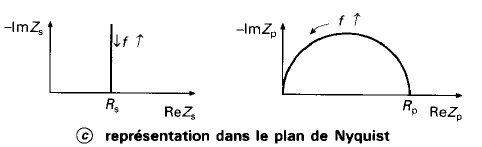
\includegraphics[keepaspectratio]{Untitled 1.png}}
\end{center}

\begin{center}
\pandocbounded{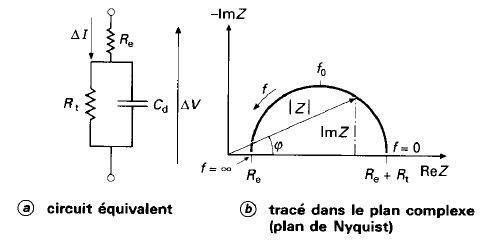
\includegraphics[keepaspectratio]{Untitled 2.png}}
\end{center}

The peak of a semi-circle (parallel RC) corresponds to the time constant
of the system \(\omega = \frac{1}{\tau} = \frac{1}{RC}\)

\begin{center}
\pandocbounded{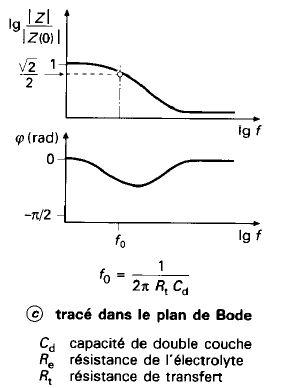
\includegraphics[keepaspectratio]{Untitled 3.png}}
\end{center}

\subsubsection{Randles Circuit}\label{randles-circuit}

\begin{center}
\pandocbounded{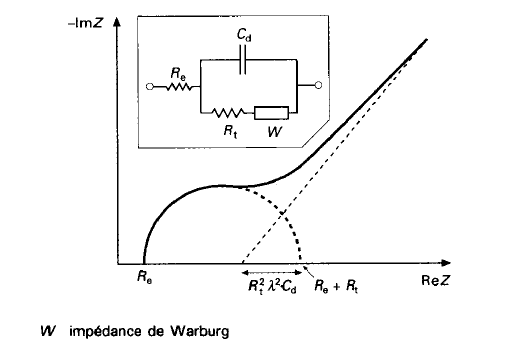
\includegraphics[keepaspectratio]{Untitled 4.png}}
\end{center}

\begin{itemize}
\tightlist
\item
  \(R_e\): Models the bulk electrolyte resistance
\item
  \(R_t\): Charge transfer resistance at the electrode-electrolyte
  interface
\item
  \(C_d\): Double-layer capacitance (charge build-up at the interface)
\item
  \(W\): Models slow diffusion processes (Warburg impedance)
\end{itemize}

\url{https://www.youtube.com/watch?v=rElEJ2UkGU0}

\url{https://www.youtube.com/watch?v=kexDd0kFAK8}

\subsection{Electrode Kinetics}\label{electrode-kinetics}

\subsubsection{Butler-Volmer}\label{butler-volmer}

\[
j = j_0 \left\{e^{\left(\frac{\alpha_a z F}{RT}(E-E_{eq})\right)} - e^{\left(-\frac{\alpha_c z F}{RT}(E-E_{eq})\right)}\right\}
\]

\[
j = j_0 \left\{e^{\left(\frac{\alpha_a z F}{RT}\eta\right)} - e^{\left(-\frac{\alpha_c z F}{RT}\eta\right)}\right\}
\]

\begin{itemize}
\tightlist
\item
  \(E\): Electrode potential
\item
  \(E_{eq}\): Equilibrium potential
\item
  \(z\): Number of electrons involved in the electrode reaction
\end{itemize}

\subsubsection{Tafel}\label{tafel}

\[
\eta = A \log\left(\frac{j}{j_0}\right)
\]

\begin{itemize}
\tightlist
\item
  \(\eta\): Overpotential
\item
  \(A\): Tafel slope
\item
  \(j\): Current density \((A/m^2)\)
\item
  \(j_0\):
  \href{https://en.wikipedia.org/wiki/Exchange_current_density}{Exchange
  current density}
\end{itemize}

The Tafel equation is an approximation of the Butler-Volmer equation at
high overpotentials \((\lvert\eta\rvert > 0.1 V)\). It assumes that the
concentrations at the electrode are practically equal to the
concentrations in the bulk electrolyte, allowing the current to be
expressed as a function of potential only. In other words, it assumes
that the electrode mass transfer rate is much greater than the reaction
rate, and that the reaction is dominated by the slower chemical reaction
rate. Also, at a given electrode the Tafel equation assumes that the
reverse half reaction rate is negligible compared to the forward
reaction rate.

\paragraph{Supporting Electrolyte}\label{supporting-electrolyte}

When performing electroanalytical experiments, it is conventional to add
a large quantity of inert salt to the solution --- this artificially
added salt is called supporting electrolyte. The purpose of the
supporting electrolyte is to increase the conductivity of the solution,
and hence to eliminate the electric field from the electrolyte.

A negligible electric field provides two advantages for electroanalysis:

\begin{itemize}
\tightlist
\item
  The voltage due to the resistance of the electrolyte when the cell
  draws current (``ohmic drop'') is minimal. Therefore, the potential
  difference applied across the electrochemical cell is localized at the
  electrode--electrolyte interfaces, and so the activation overpotential
  perceived by the redox couple at this interface is almost exactly
  proportional to the applied cell voltage. The kinetic behavior of the
  electrochemical cell then has no explicit dependence on the magnitude
  of the drawn current.
\item
  The contribution of migration to the transport of charged chemical
  species is negligible compared to the contribution of diffusion (and
  of convection, in a forced flow). Therefore the transport properties
  of the system are linearized, and they do not depend on the magnitude
  of the drawn current.
\end{itemize}

Even for the conductivities of electrolyte solutions in the presence of
excess supporting electrolyte, the electric field is not negligible if
significant current density is drawn. Electroanalysis typically draws
small currents because the purpose is measurement. In processes where an
electrochemical reaction is driven --- such as electrolysis,
electrodeposition, batteries, and fuel cells --- current densities are
typically much larger, so that the desired extent of reaction is
achieved in a reasonable time. Under these conditions, significant
electric fields are likely and other charge conservation models should
be used instead.

\paragraph{Scan Rate Influence}\label{scan-rate-influence}

The scan rate of the experiment controls how fast the applied potential
is scanned. Faster scan rates lead to a decrease in the size of the
diffusion layer; as a consequence, higher currents are
observed.\footnote{For a review see: Elgrishi, N. et al.~\emph{J. Chem.
  Educ.} 2018, 95, 197--206.} For electrochemically reversible electron
transfer processes involving freely diffusing redox species, the
Randles--Ševčík equation describes how the peak current \(i_p\) (A)
increases linearly with the square root of the scan rate \(\upsilon\) (V
s\(^{-1}\)), where \(n\) is the number of electrons transferred, \(A\)
(cm\(^2\)) is the electrode surface area, \(D_0\) (cm\(^2\) s\(^{-1}\))
is the diffusion coefficient of the oxidized analyte, and \(C^0\) (mol
cm\(^{-3}\)) is the bulk concentration of the analyte.

\[
i_p = 0.446\, nFAC^0 \left(\frac{nF\nu D_0}{RT}\right)^{\frac{1}{2}}
\]




\end{document}
